\subsection*{Teil C: Drehung und Punktspiegelung (25 Minuten)}

\begin{enumerate}[label=\arabic*.,resume]

    \item \textbf{Drehung um 90°:}

    Drehe den Punkt A(3|2) um 90° im Uhrzeigersinn um den Ursprung:

    \begin{center}
        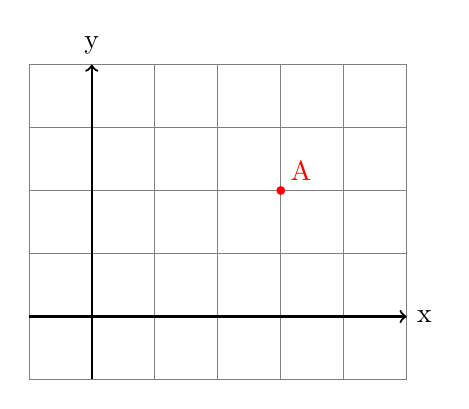
\begin{tikzpicture}[scale=0.8]
            \draw[step=1cm,gray,very thin] (-1,-1) grid (5,4);
            \draw[thick,->] (-1,0) -- (5,0) node[right]{x};
            \draw[thick,->] (0,-1) -- (0,4) node[above]{y};
            \fill[red] (3,2) circle (2pt) node[above right]{A};
        \end{tikzpicture}
    \end{center}

    Koordinaten des Bildpunktes A': (\underline{\hspace{2cm}}|\underline{\hspace{2cm}})

    \vspace{0.5cm}

    \item \textbf{Punktspiegelung:}

    Spiegle das Dreieck ABC am Punkt Z(1|1):

    A(0|3), B(2|3), C(2|0), Z(1|1)

    \begin{center}
        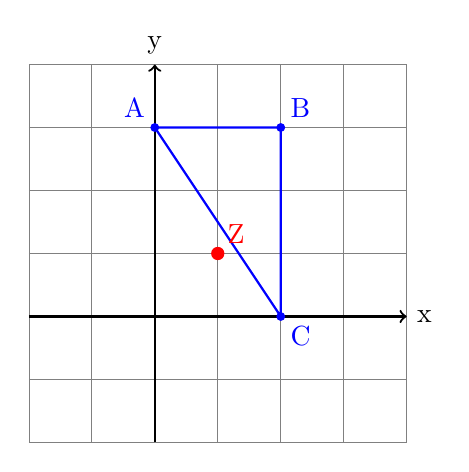
\begin{tikzpicture}[scale=0.8]
            \draw[step=1cm,gray,very thin] (-2,-2) grid (4,4);
            \draw[thick,->] (-2,0) -- (4,0) node[right]{x};
            \draw[thick,->] (0,-2) -- (0,4) node[above]{y};

            \fill[blue] (0,3) circle (2pt) node[above left]{A};
            \fill[blue] (2,3) circle (2pt) node[above right]{B};
            \fill[blue] (2,0) circle (2pt) node[below right]{C};
            \draw[blue, thick] (0,3) -- (2,3) -- (2,0) -- cycle;

            \fill[red] (1,1) circle (3pt) node[above right]{Z};
        \end{tikzpicture}
    \end{center}

    Koordinaten der Bildpunkte:
    A'(\underline{\hspace{1cm}}|\underline{\hspace{1cm}}) \hspace{1cm}
    B'(\underline{\hspace{1cm}}|\underline{\hspace{1cm}}) \hspace{1cm}  
    C'(\underline{\hspace{1cm}}|\underline{\hspace{1cm}})

    \vspace{1cm}

    \item \textbf{Vektoren drehen:}

    Drehe die Vektoren um 90°:

    \begin{tabular}{ll}
        a) $\vec{v} = \begin{pmatrix} 3 \\ 4 \end{pmatrix}$ um +90° $\rightarrow$ $\vec{v'} = \begin{pmatrix} \phantom{-3} \\ \phantom{-3} \end{pmatrix}$ & 
        b) $\vec{u} = \begin{pmatrix} 2 \\ -5 \end{pmatrix}$ um 180° $\rightarrow$ $\vec{u'} = \begin{pmatrix} \phantom{-3} \\ \phantom{-3} \end{pmatrix}$
    \end{tabular}

\end{enumerate}